\documentclass[10pt, t]{beamer}
% \usepackage[UTF8]{ctex}
\usepackage{amsmath}
\usepackage{setspace}
\usepackage{float} 
\usepackage{multido}
\usepackage{multirow}
\usepackage{array}
\usepackage{enumerate}
\usepackage{booktabs}
\usepackage{indentfirst} 
\usepackage[style=mla]{biblatex}
\usepackage{setspace}
\usepackage{subcaption}
\usepackage{hyperref}
\usepackage{textpos}
% \usepackage{fontspec}

\beamerdefaultoverlayspecification{<+->}
\makeatletter
\let\@@magyar@captionfix\relax
\makeatother

\definecolor{bladerunnerblue}{RGB}{41, 159, 163}
\definecolor{bladerunnerred}{RGB}{194,84,97}
\definecolor{themecolor}{RGB}{25,25,112} 
\definecolor{weak}{RGB}{150,150,150}

\renewcommand{\emph}[1]{{\color{themecolor}\textsl{#1}}}
\newcommand{\alarm}[1]{{\color{bladerunnerred}{#1}}}
\newcommand{\N}{\mathbb{N}}
\newcommand{\R}{\mathbb{R}}
\newcommand{\myseries}[2]{$#1_1,#1_2,\dots,#1_#2$}
\newcommand{\nullspace}{~\\[15pt]}
\newcommand{\remark}{\textbf{Remark: }}
\newcommand{\scp}[2]{\langle\,#1\,,\,#2\,\rangle} \newcommand{\scpp}{\langle\,\cdot\,,\,\cdot\,\rangle}
\newcommand{\weaken}[1]{{\color{weak}\textit{#1}}}
\newcommand{\underover}[3]{\underset{#2}{\overset{#3}{#1}}}
\renewcommand{\emptyset}{\varnothing}


\usetheme{Madrid}
\setbeamertemplate{navigation symbols}{}

\addtobeamertemplate{frametitle}{}{
\begin{textblock*}{100mm}(0.85\textwidth,-1cm)
\includegraphics[height=1cm]{../../logo.png}
\end{textblock*}}


\usecolortheme[named=themecolor]{structure}

\setbeamertemplate{items}[default]

\hypersetup{
    colorlinks=true,
    linkcolor=themecolor,
    filecolor=themecolor,      
    urlcolor=themecolor,
    citecolor=themecolor,
}

\title{VV186: Honors Mathematics}
\subtitle{\large Sequence \& Real Functions}
\institute[UM-SJTU JI]{Univerity of Michigan-Shanghai Jiao Tong University Joint Institute}
\author{Xingjian Zhang}

\begin{document}

\begin{frame}
    \titlepage
    \begin{center}
        \includegraphics[height=2cm]{../../logo2.png}
    \end{center}
\end{frame}

\begin{frame}
    \frametitle{Outline}
    \begin{spacing}{1}
        \tableofcontents
    \end{spacing}
\end{frame}

\section{Sequence}
\subsection{Cauchy Sequence}
\begin{frame}
    \frametitle{Metric \& Metric Space}
    \begin{figure}[H]
        \centering
        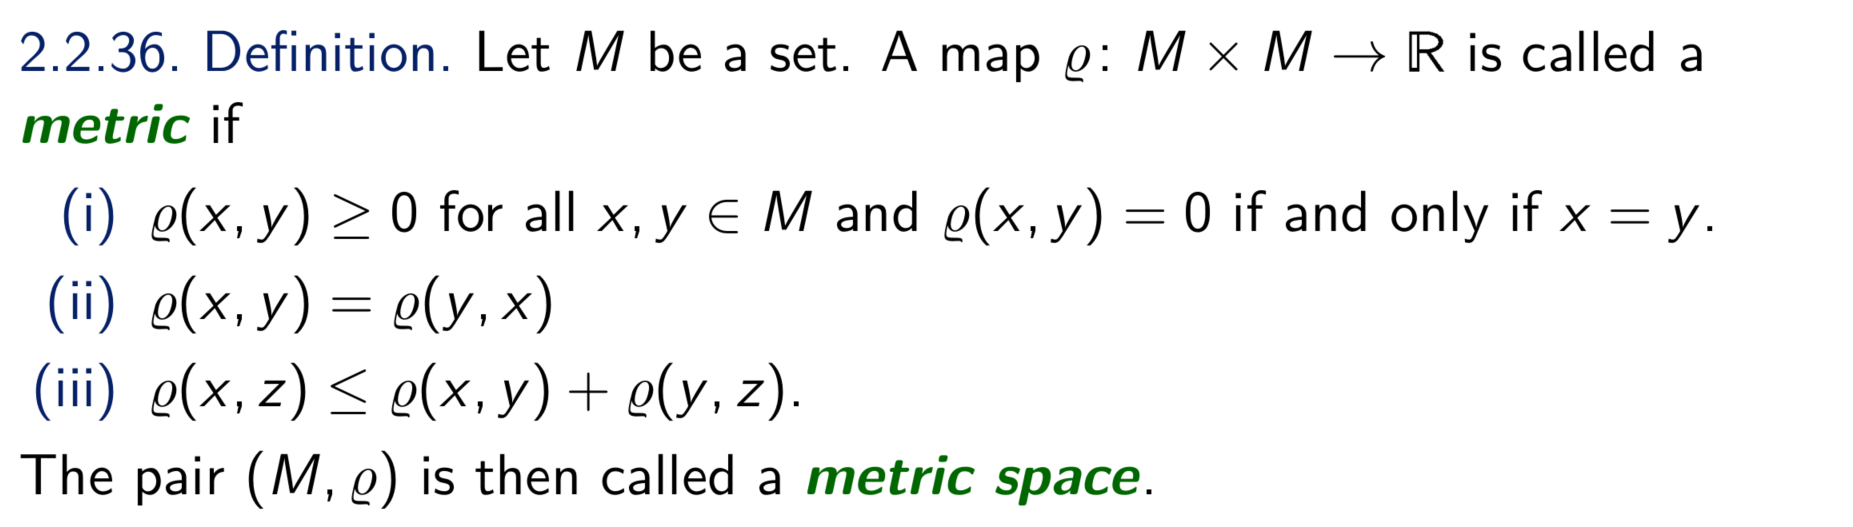
\includegraphics[width=0.9\textwidth]{2020-10-13-18-54-20.png}
    \end{figure}
    \textbf{Remark:} Metric space is a very important structure in maths. It describes how the ``distance'' between two elements in a set is measured. In the future, we will discuss a similar structure that has more nice properties: \emph{Normed Vector Space}, which is also endowed with some distance function. Try to compare metric \& norm, metric space \& normed vector space by finding their similarities \& differences (when we learn both of them).\\
\end{frame}

\begin{frame}
    \frametitle{Examples of Metric Space}

    \begin{enumerate}
        \item $\R^+$ with $d(x,y)=|\log(y/x)|$
        \item $\operatorname{Conv}(\R)$ with $d(x,y)=\sup|x-y|$. Notice that $x,y$ are real convergent sequences. (We will see this example in details later!)
        \item * \emph{The Discrete Metric.} Any set $M$ with $d(x,y)=0$ if $x=y$, $d(x,y)=1$ otherwise. This shows for any set, there is always a metric space associated with it. Moreover, by this metric, the set of any single point is an open ball (why?), and therefore every subset is open -- The space is discrete (has the \emph{discrete topology}.)
        \item * We will come back to metric space when we learn normed vector space. We will then conclude that any normed vector space is a metric space.
    \end{enumerate}

\end{frame}

\begin{frame}
    \frametitle{Generalizing Convergence}

    \begin{figure}[H]
        \centering
        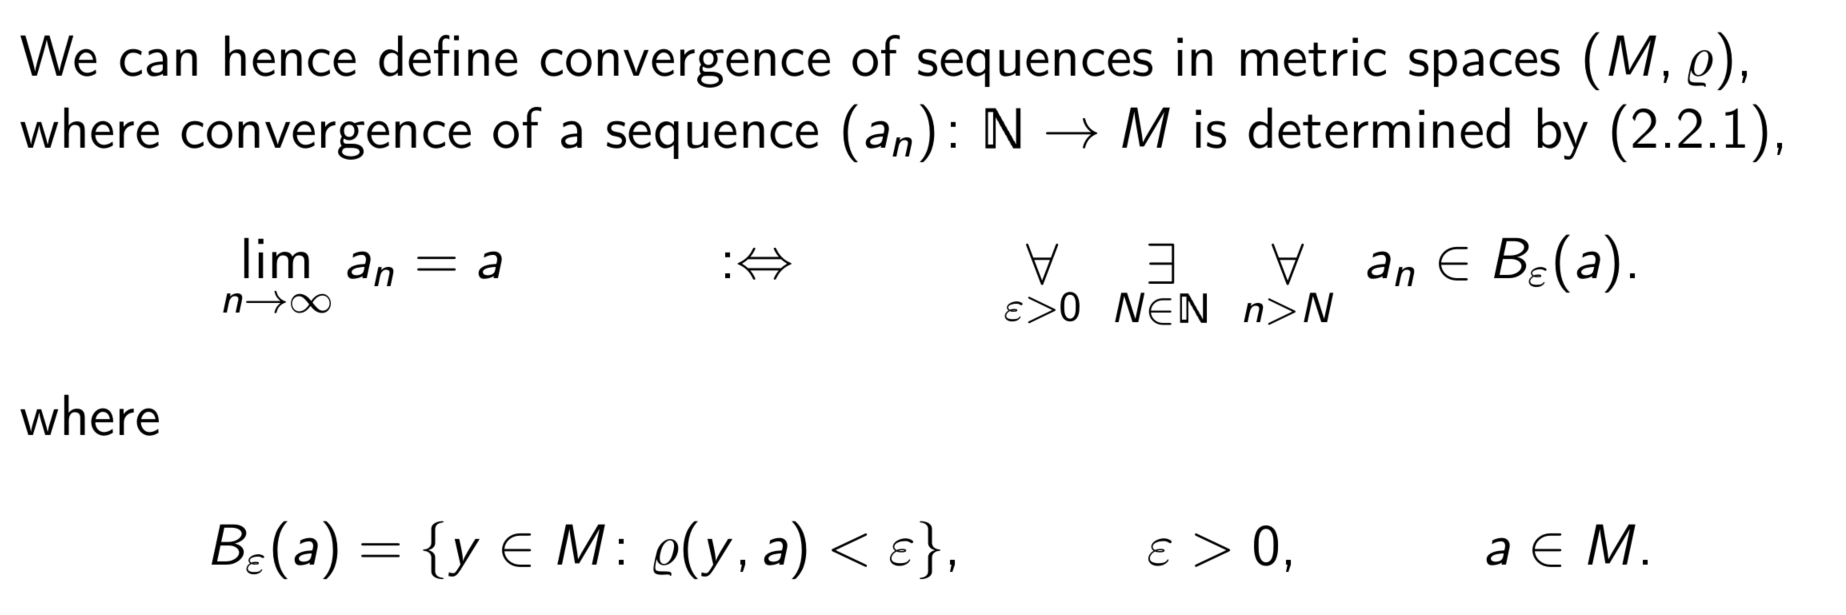
\includegraphics[width=0.9\textwidth]{2020-10-13-19-33-25.png}
    \end{figure}
    \textbf{Remark:} $B_\varepsilon(a)$ is the (generalized) \emph{open ball}. It describes the neighborhood of some element $a$ in the set $M$. (Where did we define the open ball in the previous lectures?) The open ball turns out to be an important concept in \textit{VV285}.
    \nullspace
    We then well-define the boundedness of sequence by it.
\end{frame}

\begin{frame}
    \frametitle{Cauchy Sequence}

    The fun part starts! We define the \emph{Cauchy sequences}, whose elements' distance becomes smaller and smaller:
    \begin{figure}[H]
        \centering
        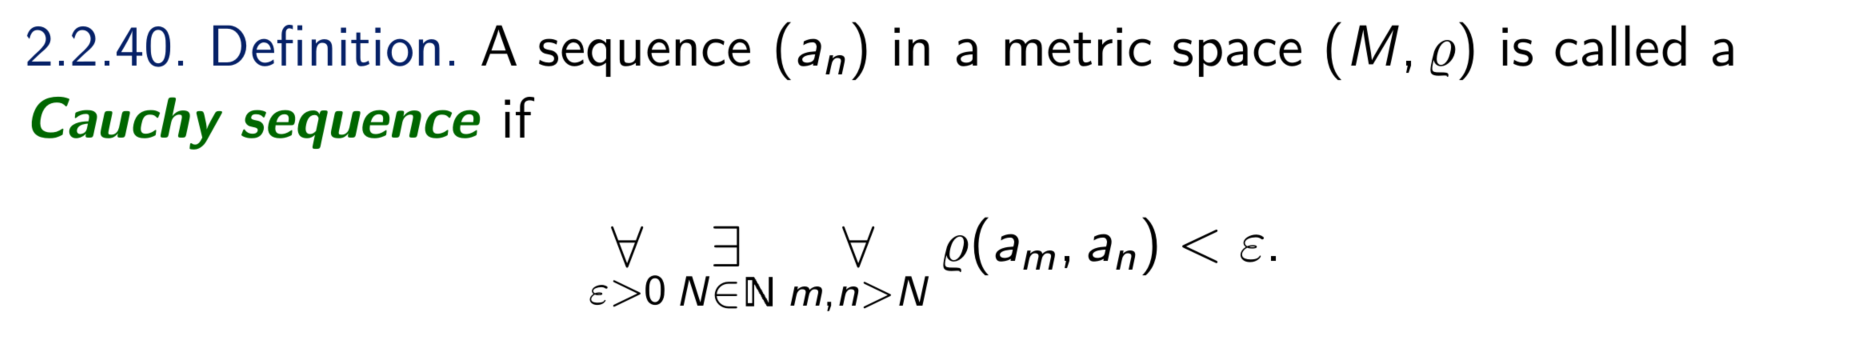
\includegraphics[width=0.9\textwidth]{2020-10-13-19-57-33.png}
    \end{figure}

    \textbf{Remark:}
    \begin{enumerate}
        \item Every Cauchy sequence is bounded.
        \item Every convergent sequence is a Cauchy sequence.
        \item However, the reverse is not necessarily true.
        \item The metric space where all Cauchy sequences converge is called a \emph{complete} metric space.
        \item A \emph{completion} of an incomplete metric space is obtained by adding all the limits of Cauchy sequences in that space. Moreover, the completion of it can be constructed as a set of \emph{equivalence classes} of Cauchy sequences in it -- That explains why Cauchy sequences are important!
    \end{enumerate}
\end{frame}

\begin{frame}
    \frametitle{A Recap on Construction of $\R$}
    \begin{figure}[H]
        \centering
        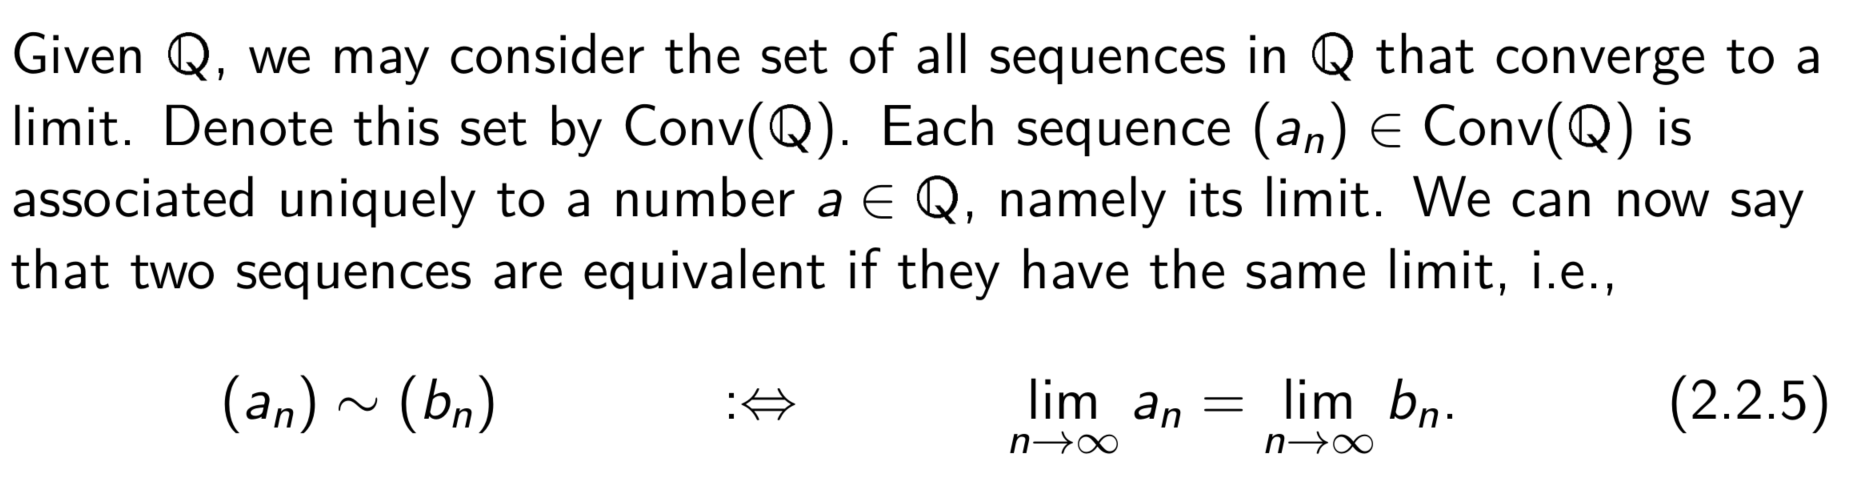
\includegraphics[width=0.9\textwidth]{2020-10-13-20-08-40.png}
    \end{figure}
    \textbf{Remark:} 
    \begin{enumerate}[<+->]
        \item $\sim $ denotes an \emph{equivalence relation} between two elements in some set.
    \end{enumerate}
\end{frame}

\begin{frame}
    \frametitle{A Recap on Construction of $\R$}
\begin{figure}[H]
        \centering
        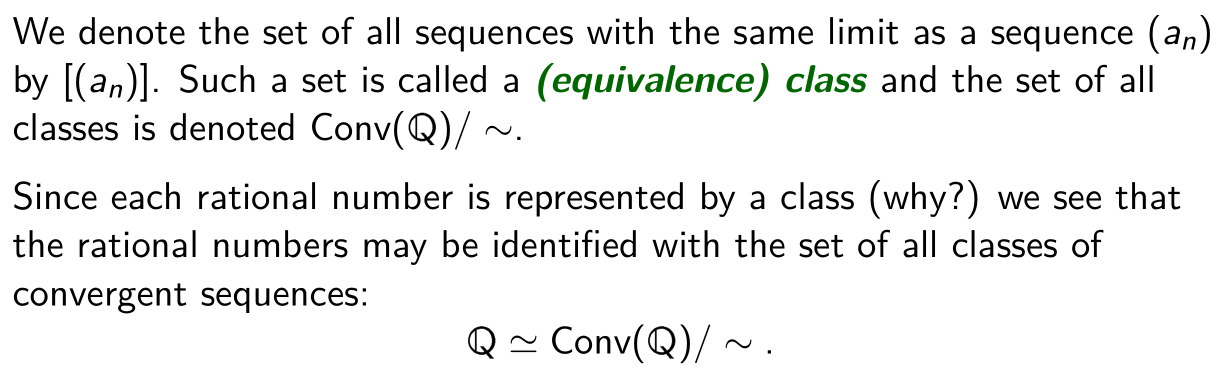
\includegraphics[width=0.9\textwidth]{2020-10-13-21-11-42.png}
    \end{figure}
    \textbf{Remark:} 
    \begin{enumerate}
        \item The equivalence relation is extremely useful in this situation. Because if $R$ is an equivalence relation on a set $M$, then for all $a,b\in M$, either $[a]\cap [b]=\emptyset$ or $[a]=[b]$. (Why? And Why is this even useful?)
        \item The equivalence classes \textbf{partition} the set $M$!
        \item $\simeq $ denotes a \emph{bijection} exists between two sets.
        \item $M/\sim$ denotes the set of all equivalence classes in $M$ \textbf{partitioned} by $\sim$.
    \end{enumerate}
\end{frame}

\begin{frame}
    \frametitle{A Recap on Construction of $\R$}
\begin{figure}[H]
        \centering
        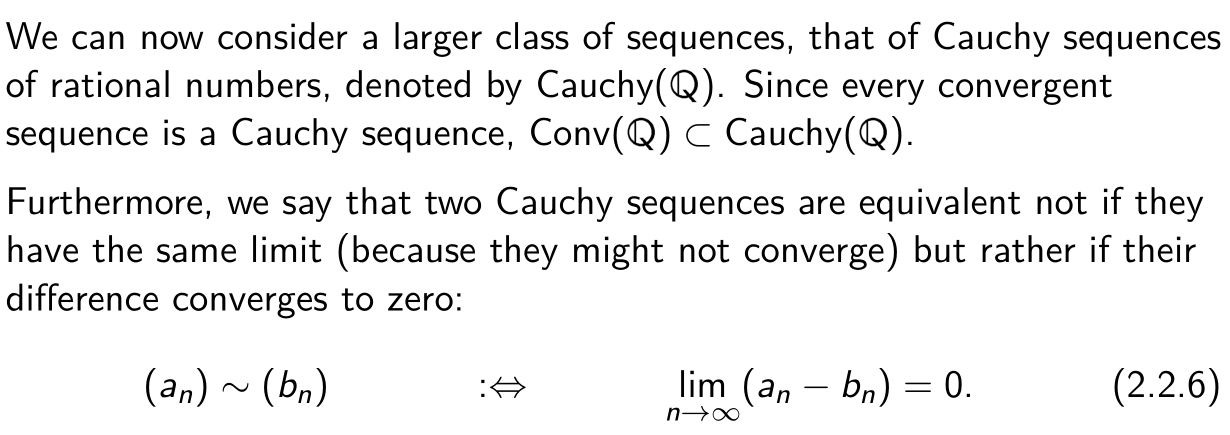
\includegraphics[width=0.9\textwidth]{2020-10-13-21-18-29.png}
    \end{figure}
    \textbf{Remark:} 
    \begin{enumerate}
        \item We define a new relationship between two Cauchy sequences, which is more general than the previous equivalence relationship.
        \item We therefore consider this $\sim$ to be a generalization of the previous $\sim$ -- So we reuse the same symbol.
        \item Finally, we have a larger set:
        $$\operatorname{Cauchy}(\mathbb{Q}) / \sim \supset \operatorname{Conv}(\mathbb{Q}) / \sim \simeq \mathbb{Q}$$
    \end{enumerate}
\end{frame}

\begin{frame}
    \frametitle{A Recap on Construction of $\R$}
\begin{figure}[H]
        \centering
        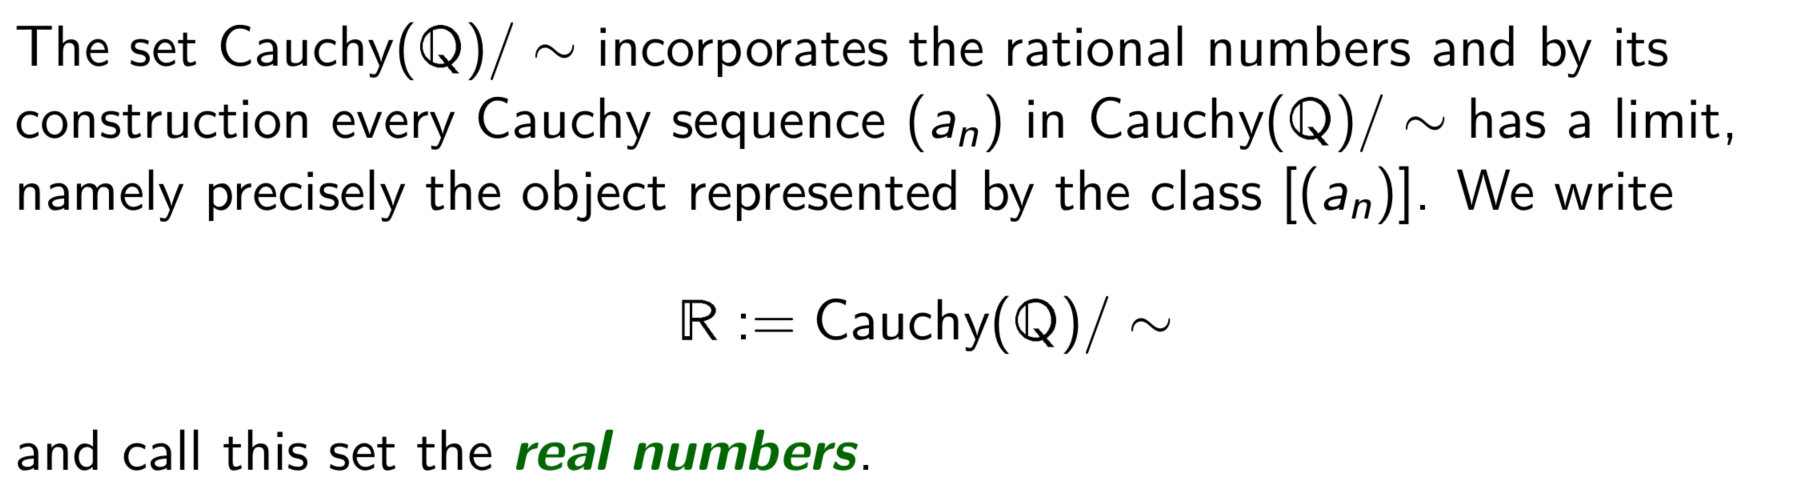
\includegraphics[width=0.9\textwidth]{2020-10-13-21-23-38.png}
    \end{figure}
    \textbf{Remark:} 
    \begin{enumerate}
        \item We then \textbf{define} the set of real numbers to be this larger set. 
        \item Recall how did we construct the natural numbers $\N_{def}$? Sets!
    \end{enumerate}
\end{frame}

\begin{frame}
    \frametitle{Regarding $\simeq$}

    A way to think about $\simeq$, a bijection exists between two sets $A$ and $B$, is that the abstract entities  $A$ and $B$ are equivalent and \textbf{essentially the same} -- they are both sets, so they contain no information about repetition or order, and since there is a bijection between them, we can obtain one from the other simply by relabeling the elements.
    \nullspace
    To some extent, this also explains why we use other abstraction to construct natural numbers or real numbers: we are looking for a correspondence between a known concept and a new concept.
    \nullspace
    * An explicit definition will be given in VE203.\footnote[frame]{*Morphisms and Isomorphisms.}

\end{frame}

\begin{frame}
    \frametitle{Example of Abstract Incomplete Metric Space}
    Let's see one abstract metric space that is not complete.\\[8pt] We define the set of all real sequences that vanish from some points to be $U$. i.e.
    $$U=\{(a_n)|\exists N\in\N,\forall n>N:a_n=0\}.$$
    It is clear that $U\subset c_0$, where $$c_0=\{(a_n)|\lim a_n = 0\}.$$
    We use the metric $$\rho((a_n),(b_n))=\sup|a_n-b_n|.$$
    Define a sequence of sequences $(a_n^{(N)})\in U$, $$(a_n^{(N)})=\left\{\begin{matrix}
        \dfrac{1}{n},\, n\leq N\\[8pt]
        0,\, n>N
        \end{matrix}\right.$$
    Is $(a_n^{(N)})$ a Cauchy sequence in $(U,\rho)$? Does $(a_n^{(N)})$ has a limit in this space? What is the completion of $(U,\rho)$?

\end{frame}

\begin{frame}
    \frametitle{Exercise}

    % find some exercise here

\end{frame}

\begin{frame}
    \frametitle{End}
    \vspace{2.2cm}
    \begin{center}
        \Large
        Have Fun \\
        And \\
        Learn Well!\footnote[frame]{Special acknowledgement to former TA Zhang Leyang, who offered many exercises and advice to my recitation class.}
    \end{center}
\end{frame}

\end{document}